% details of models used for re-analysis of Hutchings and Baum
% Daniel Ricard
% Date last modified Time-stamp: <2009-08-05 13:46:55 (ricardd)>

\documentclass[letterpaper,12pt]{article}

\usepackage{graphicx}

\title{Modelling details for biomass time trends analyses}
\author{D. Ricard \and C. Minto}
\begin{document}
\maketitle



\section{Model details}
To determine the difference in temporal trend before and after a cutoff date, we model the biomass of a species as:

\begin{equation}
log\left(B\right) = \left[ \alpha_{0} + \left(\delta_{post}^{\alpha} * post\right)\right] + \left[ \beta_{0} + \left(\delta_{post}^{\beta} * post\right) \right]yr
\end{equation}
where,
\begin{description}
\item{$\alpha_{0}$} is the overall intercept
\item{$\delta_{post}^{\alpha}$} is the deviation from the overall intercept after the cutoff year
\item{$\beta_{0}$} is the overall slope
\item{$\delta_{post}^{\beta}$} is the deviation from the overall slope after the cutoff year
\item{$post$} determines whether the year $yr$ is before ($post=0$) or after ($post=1$) the cutoff year
\end{description}

The benefits of this model are that the value of $\delta_{post}^{\alpha}$ determines the change in biomass between the beginning of the time-series and the cutoff date. The value of $\delta_{post}^{\beta}$ determines whether the biomass time trend has changed after the cutoff date. To test the applicability of this model, we test it on five simulated data sets with the following characteristics:

\begin{enumerate}
\item{Steady decrease in biomass over time}
\item{Steady increase in biomass over time}
\item{Decrease in biomass over time until the cutoff date, followed by a steady increase in biomass}
\item{Decrease in biomass over time until the cutoff date, followed by no change in biomass}
\item{No change in biomass over time}
\end{enumerate}

Simulated datasets can be found in Figure~\ref{fig:sim} with model fits overlaid. 
% Parameter estimates for model fits can be found in Table~\ref{tab:simfits}.

The proposed model properly captures the simulated trends and provides an appropriate methodology to evaluate stock recoveries.

\begin{figure}[htb]
 \begin{center}
 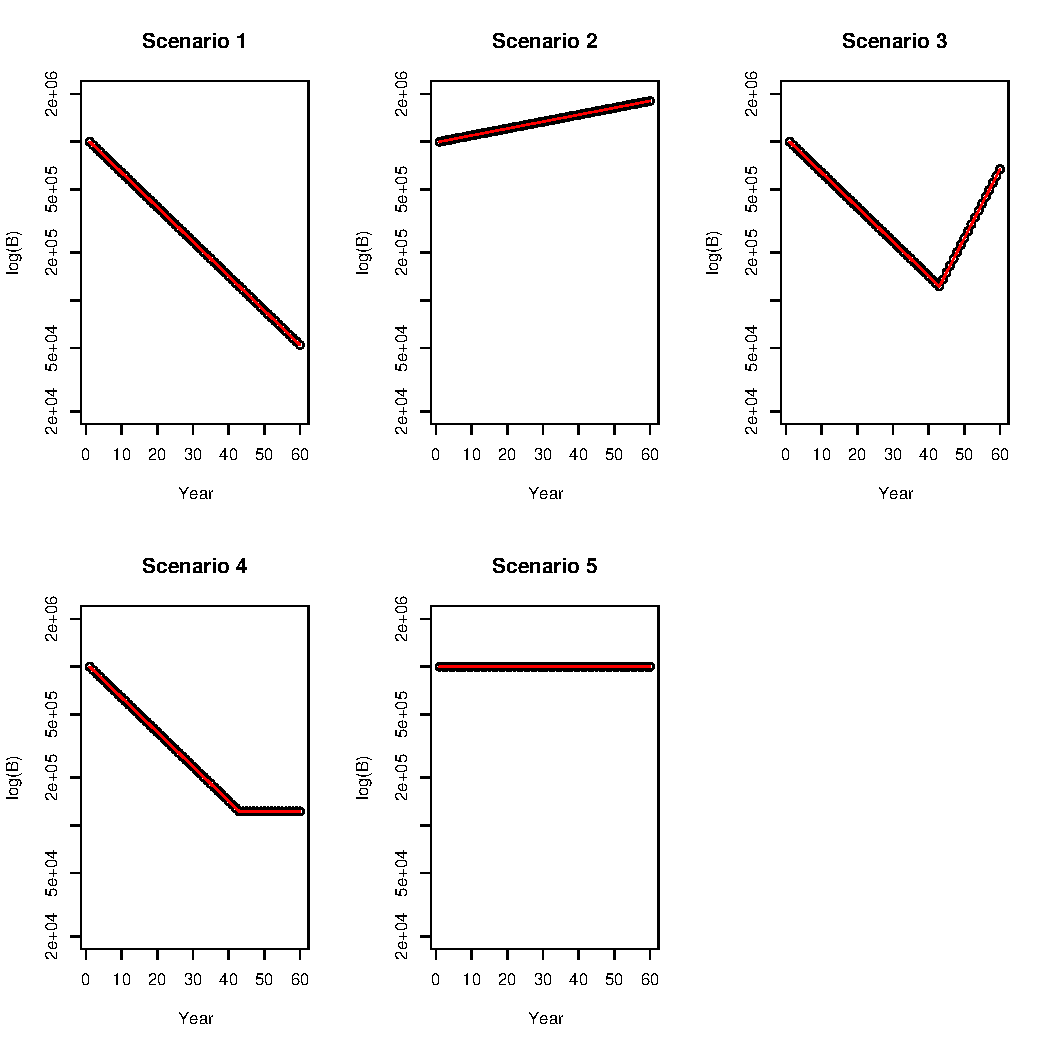
\includegraphics[scale=0.65]{../R/sim.pdf}
 \end{center}
 \caption{Simulated datasets (black dots) and model fits (red lines).}\label{fig:sim}
\end{figure} 

%\begin{table}[htbp]
% \begin{tabular}{l|l|l}
% Scenario & Simulated & Fitted \\ \hline \hline
%1 & $\alpha_{0}=13.81551$, $\beta_{0}=-0.05$, $\delta_{post}^{\beta}=0$ & $\alpha_{0}=13.86551$, $\beta_{0}=-0.05$, $\delta_{post}^{\beta}=0$ \\
%2 & $\alpha_{0}=13.81551$, $\beta_{0}=0.01$, $\delta_{post}^{\beta}=0$ & $\delta_{post}^{\beta}=0$ \\
%3 & $\alpha_{0}=13.81551$, $\beta_{0}=-0.05$, $\delta_{post}^{\beta}=0.15$ & $\delta_{post}^{\beta}=0.15$ \\
%4 & $\alpha_{0}=13.81551$, $\beta_{0}=-0.05$, $\delta_{post}^{\beta}=0.05$ & $\delta_{post}^{\beta}=0.05$ \\
%5 & $\alpha_{0}=13.81551$, $\beta_{0}=0$, $\delta_{post}^{\beta}=0$ & $\delta_{post}^{\beta}=0$ \\
% \end{tabular} 
%\caption{Parameter values used to simulate the data and parameter estimates from model fits.}\label{tab:simfits}
%\end{table} 

\section{Proposed analyses}

Time-series of biomass will be extracted from the updated stock-recruitment database and the above model will be fit for all available stocks. Parameter estimates will determine 1) the magnitude of decline between the first year of data and 1992, and 2) whether the temporal trend has changed since 1992.

Other analyses will also be conducted, with the overall aim to reproduce the analyses presented in Hutchings and Baum 2005 paper.

\end{document}